\documentclass[letterpaper,12pt,fleqn]{article}
\usepackage{matharticle}
\usepackage{pgfplots}
\pgfplotsset{compat=1.14}
\pagestyle{plain}
\begin{document}

\begin{center}
\Large Math-1003b Practice Exam \#2
\end{center}

\vspace{0.5in}

This exam is closed book and notes. You may use a scientific calculator; however, no
other electronics are allowed. Show all work; there is no credit for guessed answers. All
answers must be in factored form, where appropriate. All numerical answers must be
expressed using exact values, unless you are specifically asked for an approximate
(decimal) value. All intervals must be expressed in interval notation.

\vspace{0.25in}

\begin{enumerate}
\item A company makes metal pipe for the plumbing industry. The cost to make a particular
  type of pipe varies directly with the length of the pipe and inversely with the
  diameter of the pipe (smaller pipes are harder to make).
  \begin{enumerate}
  \item Let $p=$ the cost to make each pipe, $L=$ length of each pipe and $d=$ diameter of
    each pipe. Write an equation that expresses the cost of each pipe in terms of $L$
    and $d$.

  \item What is the value of the constant of proportionality if the cost per pipe is
    80 cents when making a 2 foot pipe with a diameter of half an inch?

  \item What is the cost per pipe for a 5 foot pipe with a 2 inch diameter?
  \end{enumerate}

\item Solve the compound inequality for $x$:
  \[-6\le-5(x+1)+4<9\]

\item Solve the following system of inequalities for $x$:
  \[x-1\ge3\hspace{2ex}\mbox{or}\hspace{2ex}-2(x-5)<6\]

\item Solve for $x$ using test points:
  \[x^2+7x-18>0\]

\item Solve for $x$ using test points:
  \[\frac{x-5}{x+2}\le0\]

\item Solve for $x$:
  \[3\abs{2x+1}-1=8\]

\item Solve for $x$:
  \[\abs{3x-1}=-2\]

\item Solve for $x$:
  \[3\abs{4x+1}-5<7\]

\item Solve for $x$ (Hint: Look at the previous problem):
  \[3\abs{4x+1}-5\ge7\]

\item Solve the following system of inequalities by graphing. Be sure to label all key
  points and make it absolutely clear which region(s) of the plane you are selecting for
  your answer:
  \[\left\{\begin{array}{l} y\ge-1 \\ x-y<2 \end{array}\right.\]
  
  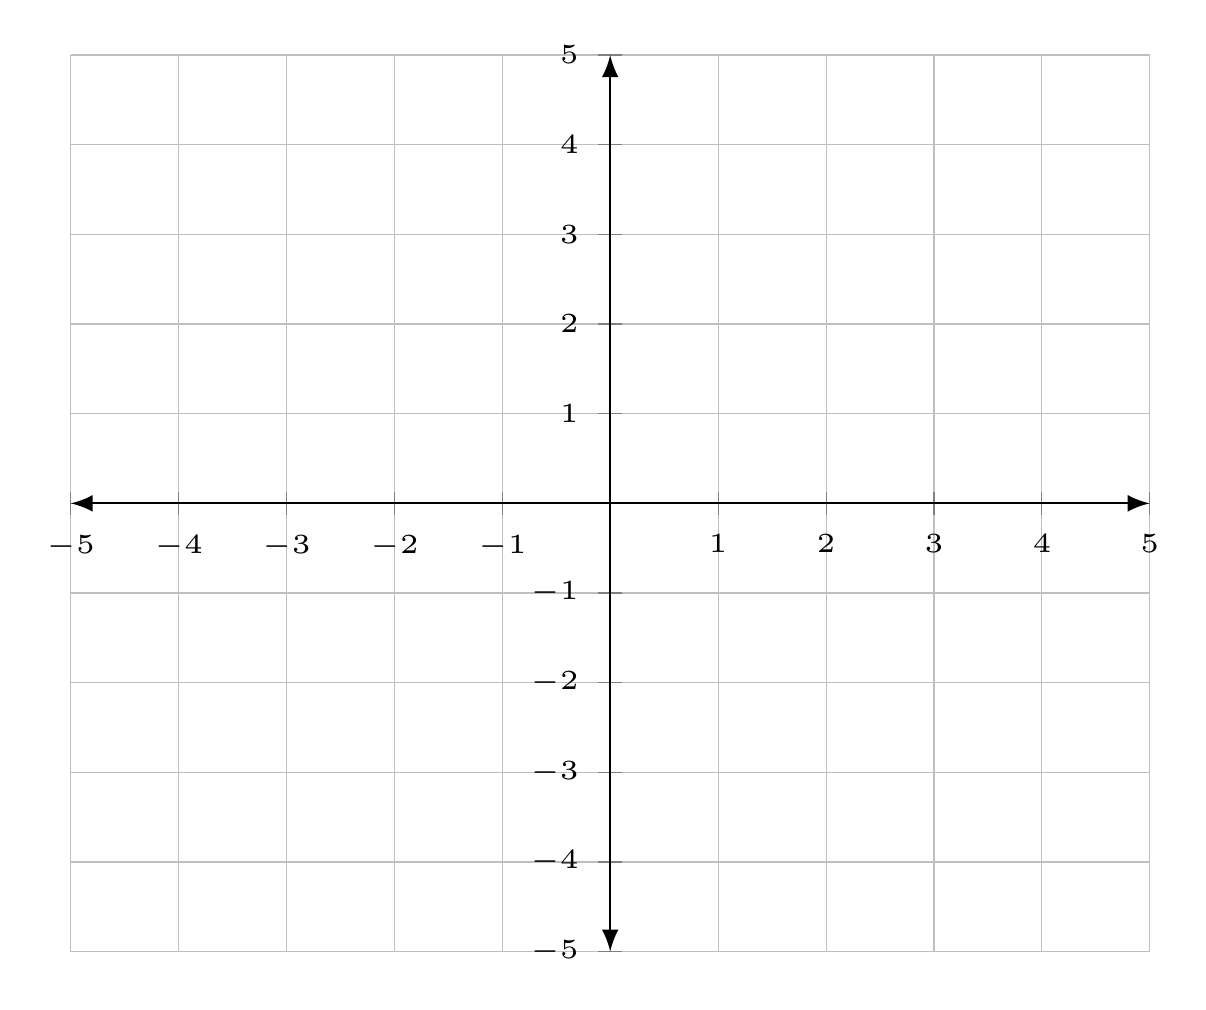
\begin{tikzpicture}[scale=2]
    \begin{axis}[
        xmin=-5,xmax=5,
        ymin=-5,ymax=5,
        grid=both,
        grid style={line width=.1pt, draw=gray!10},
        major grid style={line width=.2pt,draw=gray!50},
        axis lines=middle,
        axis line style={latex-latex},
        xtick={-5,-4,-3,-2,-1,0,1,2,3,4,5},
        ytick={-5,-4,-3,-2,-1,0,1,2,3,4,5},
        ticklabel style={font=\tiny},
      ]
    \end{axis}
  \end{tikzpicture}

\end{enumerate}

\end{document}
